
\section{Results \label{sec:results_compliant}}









In this section, we present the simulation tests of the control strategy presented in Section~\ref{sec:controller_tsid_compliant}.
The proposed strategy is also compared with the task-based inverse dynamics algorithm that considers rigid contacts presented in Section~\ref{sec:dynamics_QP}. From now on, the proposed control approach is called \emph{TSID-Compliant}, and the controller of Section~\ref{sec:dynamics_QP} \emph{TSID-Rigid}.
The experiments are carried out on a simulated version of the humanoid robot iCub v2.7~\citep{Metta2010} -- Section~\ref{sec:icub2.7}. The architecture takes (on average) less than $\SI{1}{\milli \second}$ to evaluate its outputs. The OSQP~\citep{Stellato2018} library is used to solve the optimization problems. The code is open source it is available at \href{https://github.com/ami-iit/Romualdi-2021-RAL-soft\_terrain\_walking}{\texttt{https://github.com/dic-iit/Romualdi-2021-RAL-soft\_terrain\_walking}}.
Simulations are obtained by integrating the robot forward dynamics (FD) obtained from~\eqref{eq:system_initial}. Figure~\ref{fig:block-diagram-compliant} shows the connection between the whole-body controller the contact parameter estimator and the simulator. The FD is evaluated with the contact model in Lemma~\ref{lemma:compliant_model} perturbed with a zero-mean Gaussian noise.
\par
To validate the performance of the proposed architecture, we present three main experiments.
First, we compare the performances of the TSID-Compliant and the TSID-Rigid controllers in case of different contact parameters. Second, we analyze the robustness of the TSID-Compliant in case of non-parametric uncertainty in the contact model. Finally, we show the contact parameter estimation performances in case of anisotropic environment. In all scenarios, the robot walks straight and the maximum velocity is $\SI{0.17}{\meter \per \second}$.
\begin{figure}[t]
        \begin{subfigure}[b]{0.32\textwidth}
        \centering
        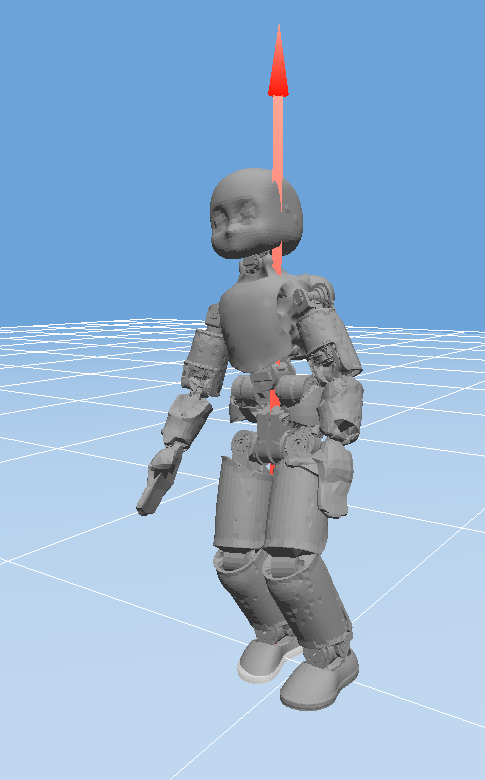
\includegraphics[width=\columnwidth]{chapter_compliant_contact/figures/step1.png}
    \end{subfigure}
    \hfill
    \begin{subfigure}[b]{0.32\textwidth}
        \centering
        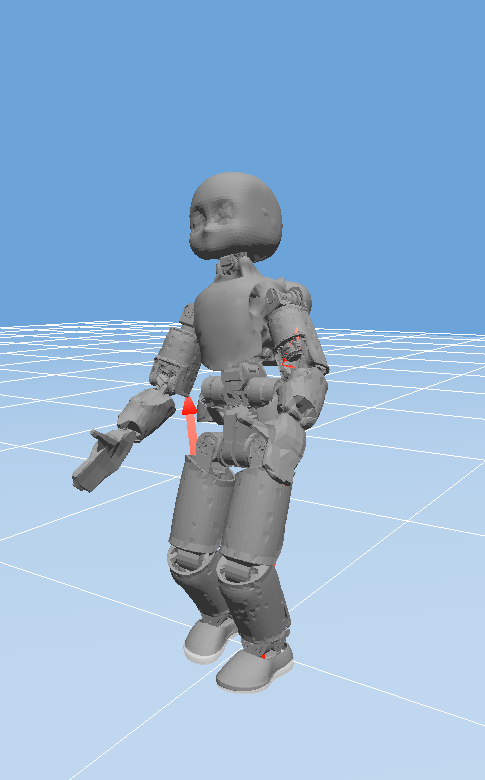
\includegraphics[width=\columnwidth]{chapter_compliant_contact/figures/step2.png}
    \end{subfigure}
    \hfill
     \begin{subfigure}[b]{0.32\textwidth}
        \centering
        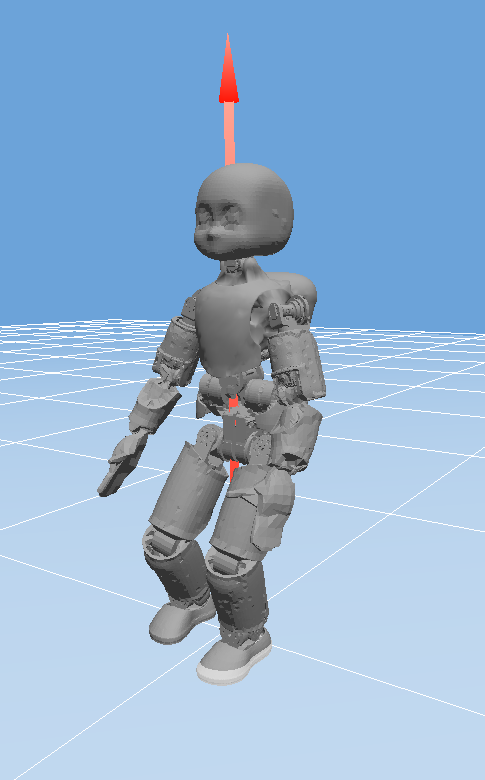
\includegraphics[width=\columnwidth]{chapter_compliant_contact/figures/step3.png}
    \end{subfigure}
    \caption{A simulation of the iCub robot walks with the TSID-Compliant controller.}
\end{figure}

\subsection{Comparison between TSID-Compliant and TSID-Rigid}
Table~\ref{tab:architecture_outcome} summarizes the outcome of the control strategies for different contact parameters. Labels \emph{success} and \emph{failure} mean that the associated controller is able or not to ensure that the robot is balanced while walking.

\begin{table}[!b]
    \centering
    \caption{Outcomes of whole-body controllers implementation on compliant terrain walking.
    }
    \begin{tabular}{c|c|c|c}
         \begin{tabular}{@{}c@{}}\textbf{TSID Type}\end{tabular} &
         \begin{tabular}{@{}c@{}}\textbf{k (N/m${}^{\mathbf{3}}$)} \end{tabular} &
         \begin{tabular}{@{}c@{}}\textbf{b (Ns/m${}^{\mathbf{3}}$)}\end{tabular} &
         \begin{tabular}{@{}c@{}}\textbf{Outcome}\end{tabular}\\
        \hline
        Compliant  & $\SI{8e5}{}$  &  $\SI{1e4}{}$ & Success \\
        \hline
        Compliant  & $\SI{1e6}{}$  &  $\SI{1e4}{}$ & Success \\
        \hline
        Compliant  & $\SI{2e6}{}$  &  $\SI{1e4}{}$ & Success \\
        \hline
        Compliant  & $\SI{8e5}{}$  &  $\SI{1e3}{}$ & Success \\
        \hline
        Compliant  & $\SI{2e6}{}$  &  $\SI{1e3}{}$ & Success \\
        \hline
        Compliant  & $\SI{1e6}{}$  &  $\SI{1e3}{}$ & Success \\
        \hline
        Rigid  & $\SI{8e5}{}$  &  $\SI{1e4}{}$ & Failure \\
        \hline
        Rigid  & $\SI{1e6}{}$  &  $\SI{1e4}{}$ & Failure \\
        \hline 
        Rigid  & $\SI{2e6}{}$  &  $\SI{1e4}{}$ & Success \\
        \hline 
        Rigid  & $\SI{8e5}{}$  &  $\SI{1e3}{}$ & Failure \\
        \hline 
        Rigid  & $\SI{1e6}{}$  &  $\SI{1e3}{}$ & Failure \\
        \hline
        Rigid  & $\SI{2e6}{}$  &  $\SI{1e3}{}$ & Failure \\
    \end{tabular}
    \label{tab:architecture_outcome}
\end{table}
\par
To compare the two controllers, we decided to perform three main experiments. In the first experiment, we choose a set of contact parameters such that both whole-body controllers guarantee balance while walking. In the second, we keep the damper coefficient $b$ constant, and we decrease the spring coefficient $k$. Finally, in the third experiment, we keep $k$ constant and decrease $b$.  Namely: 
\begin{itemize}
    \item[\textbf{-}]\textbf{Experiment 1} $k=\SI{2e6}{\newton \per \meter^3}$, $b = \SI{1e4}{\newton \second \per \meter^3}$;
    \item[\textbf{-}]\textbf{Experiment 2} $k=\SI{1e6}{\newton \per \meter^3}$, $b=\SI{1e4}{\newton \second \per \meter^3}$;
    \item[\textbf{-}]\textbf{Experiment 3} $k = \SI{2e6}{\newton \per \meter^3}$, $b=\SI{1e3}{\newton \second \per \meter^3}$.
\end{itemize}


\begin{figure}[t]
    \begin{myframe}{k = $\SI{2e6}{\newton \per \meter^3}$  b = $\SI{1e4}{\newton \second \per \meter^3}$}
    \centering
        \begin{subfigure}[b]{0.49\textwidth}
        \centering
        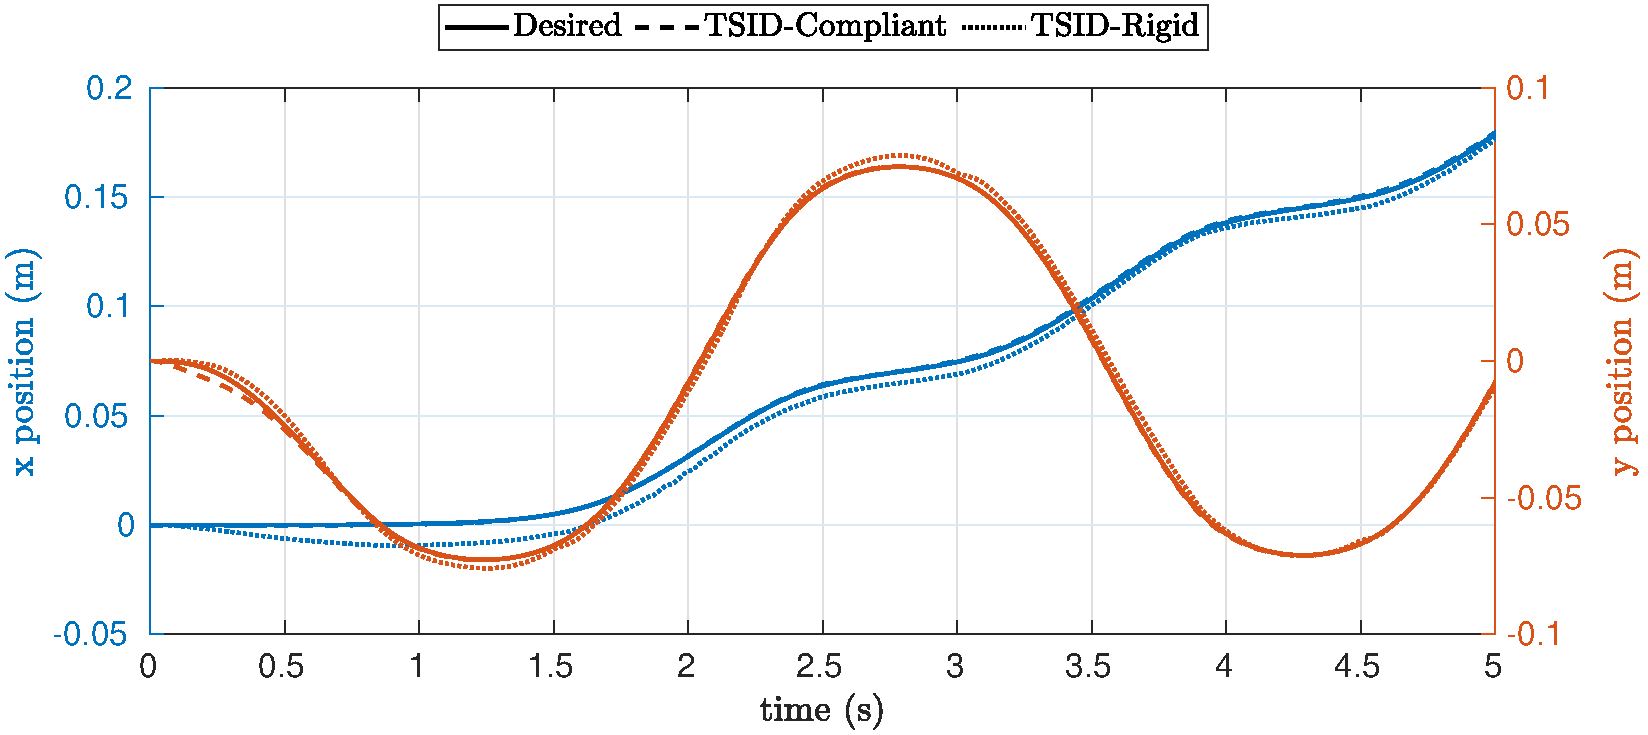
\includegraphics[height=0.151\textheight]{chapter_compliant_contact/figures/compliant_2e6_1e4_stiff_2e6_1e4_com.pdf}
        \caption{CoM}
        \label{fig:2e6_1e4_com}
    \end{subfigure}
    \hfill
    \begin{subfigure}[b]{0.49\textwidth}
        \centering
        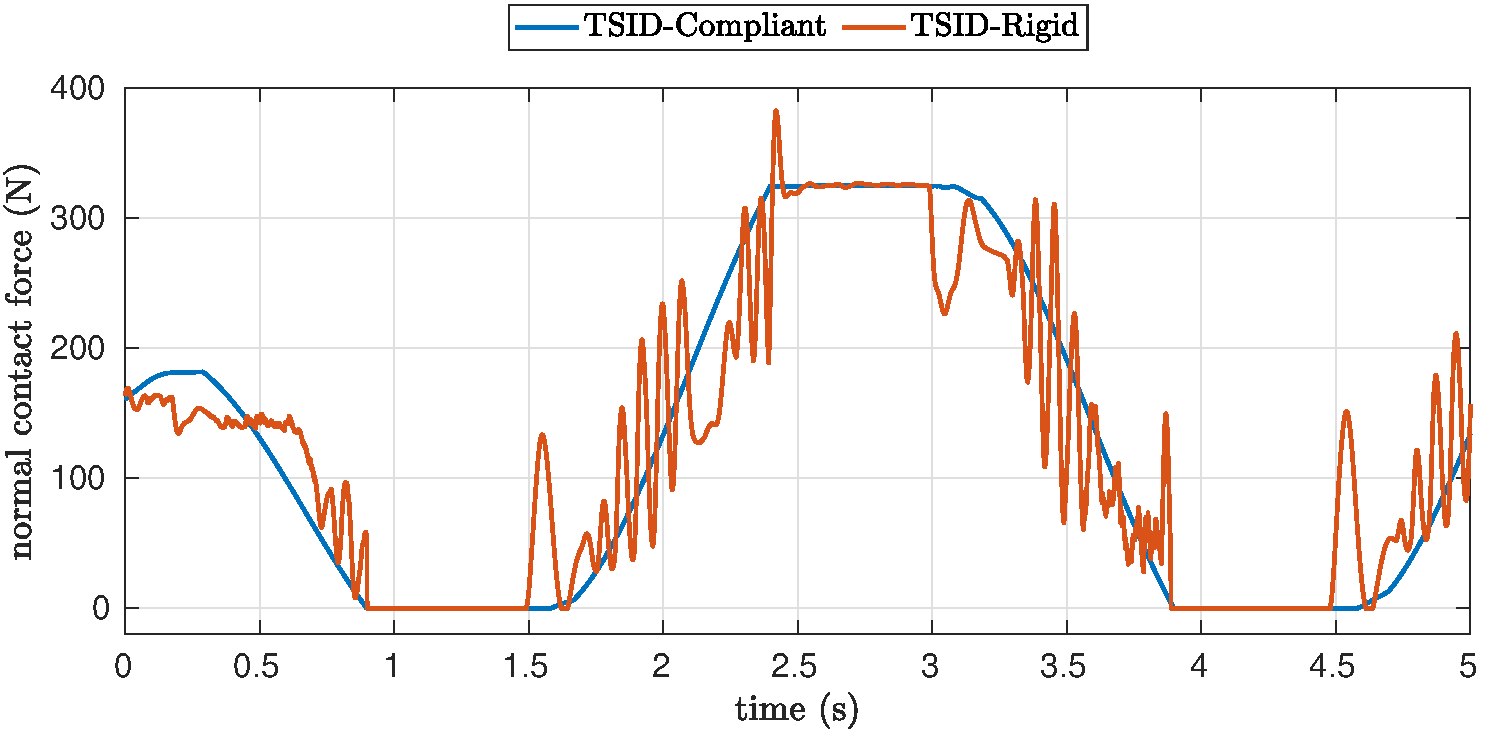
\includegraphics[height=0.151\textheight]{chapter_compliant_contact/figures/compliant_2e6_1e4_stiff_2e6_1e4_force.pdf}
        \caption{Normal contact force}
        \label{fig:2e6_1e4_force}
    \end{subfigure}
     \begin{subfigure}[b]{0.49\textwidth}
        \centering
        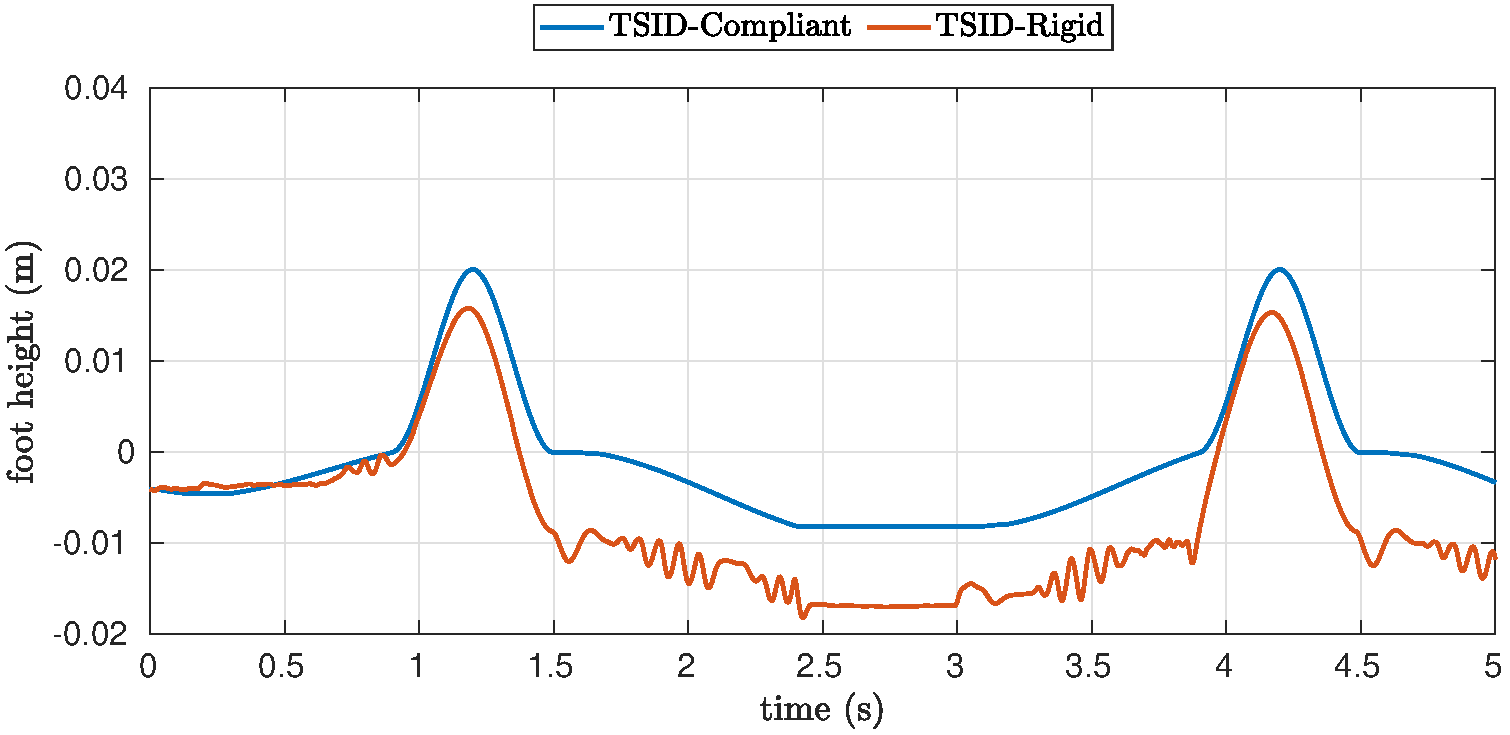
\includegraphics[height=0.151\textheight]{chapter_compliant_contact/figures/compliant_2e6_1e4_stiff_2e6_1e4_foot.pdf}
        \caption{Foot trajectory}
        \label{fig:2e6_1e4_foot}
    \end{subfigure}
    \end{myframe}
    \caption{Comparison between TSID-Rigid and TSID-Compliant.}
\end{figure}

\begin{figure}[t]
    \begin{myframe}{k = $\SI{2e6}{\newton \per \meter^3}$  b = $\SI{1e3}{\newton \second \per \meter^3}$}
    \centering
        \begin{subfigure}[b]{0.49\textwidth}
        \centering
        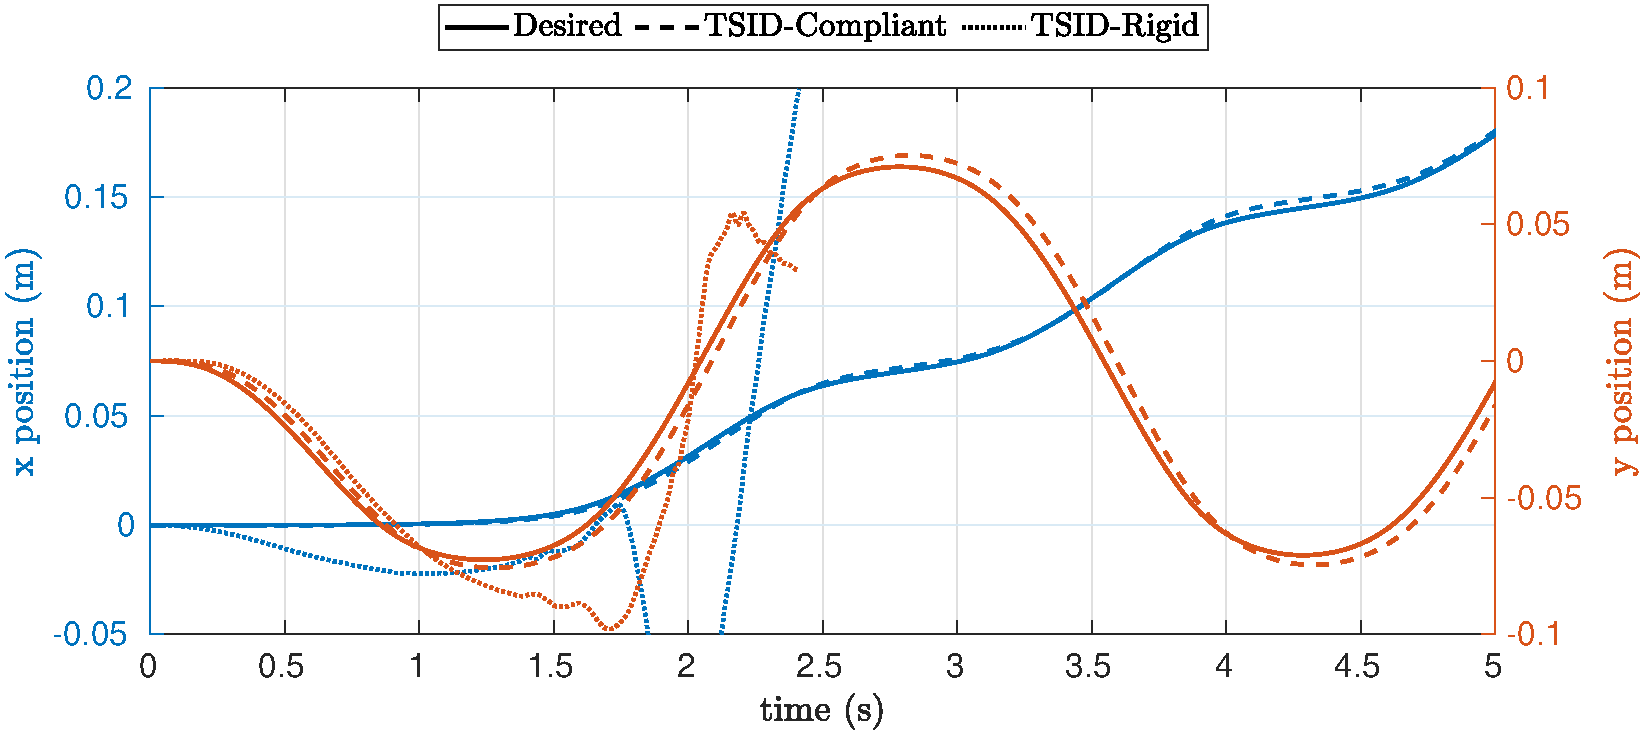
\includegraphics[height=0.151\textheight]{chapter_compliant_contact/figures/compliant_2e6_1e3_stiff_2e6_1e3_2_com.pdf}
        \caption{CoM}
        \label{fig:2e6_1e3_com}
    \end{subfigure}
    \hfill
    \begin{subfigure}[b]{0.49\textwidth}
        \centering
        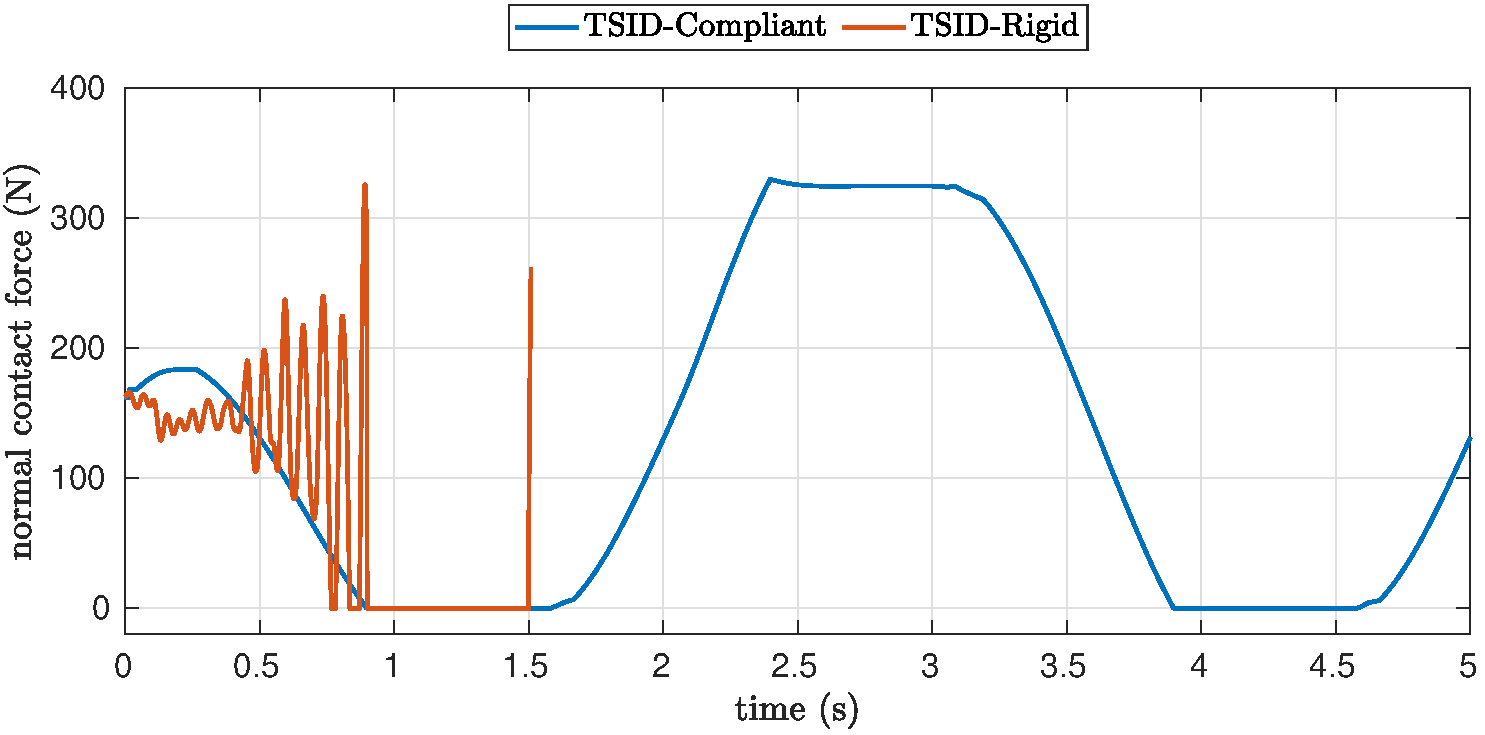
\includegraphics[height=0.151\textheight]{chapter_compliant_contact/figures/compliant_2e6_1e3_stiff_2e6_1e3_2_force.pdf}
        \caption{Normal contact force}
        \label{fig:2e6_1e3_force}
    \end{subfigure}
     \begin{subfigure}[b]{0.49\textwidth}
        \centering
        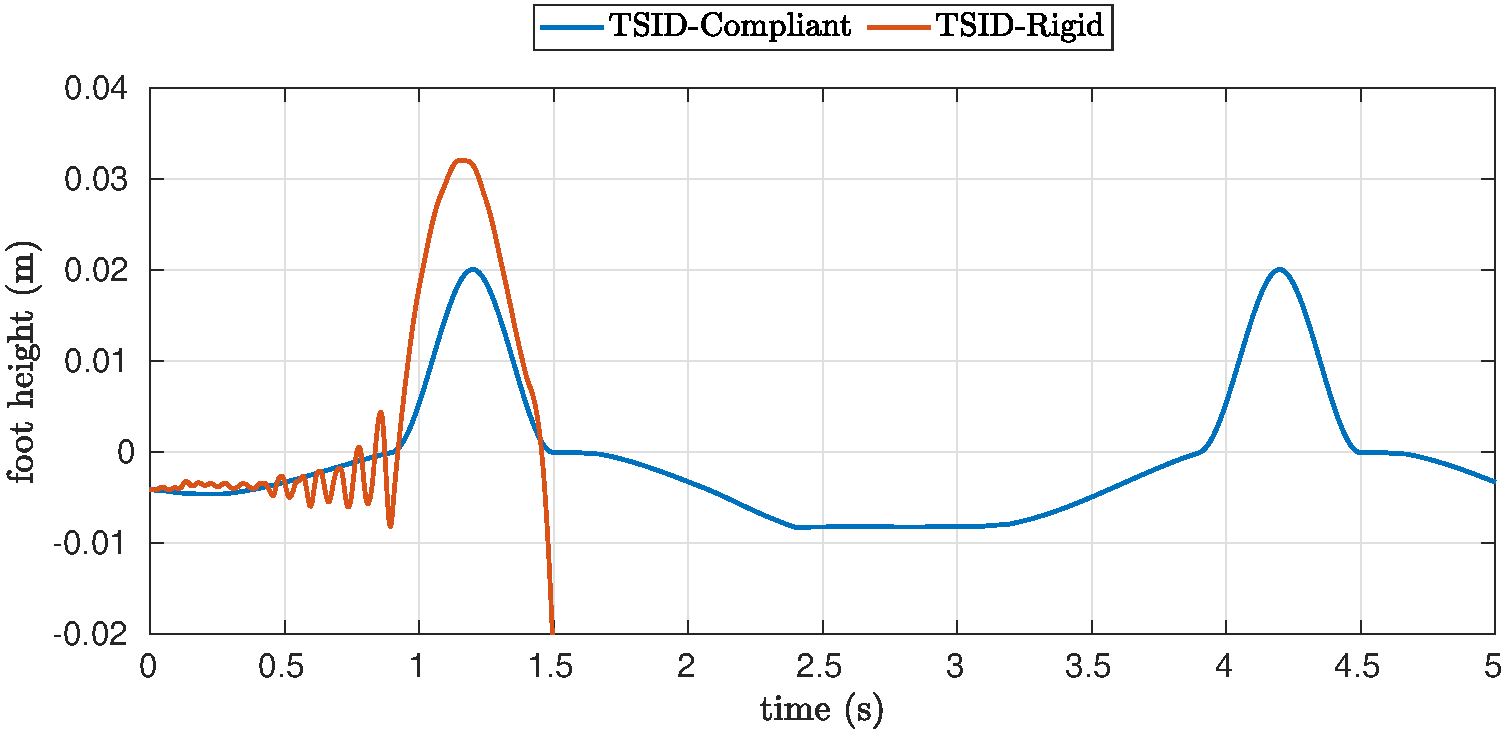
\includegraphics[height=0.151\textheight]{chapter_compliant_contact/figures/compliant_2e6_1e3_stiff_2e6_1e3_2_foot.pdf}
        \caption{Foot trajectory}
        \label{fig:2e6_1e3_foot}
    \end{subfigure}
    \end{myframe}
    \caption{Comparison between TSID-Rigid and TSID-Compliant. At $t\approx \SI{1.75}{\second}$, the TSID-Rigid makes the robot fall down.}
\end{figure}

\begin{figure*}[!t]
    \begin{myframe}{k = $\SI{1e6}{\newton \per \meter^3}$  b = $\SI{1e4}{\newton \second \per \meter^3}$}
    \centering
        \begin{subfigure}[b]{0.49\textwidth}
        \centering
        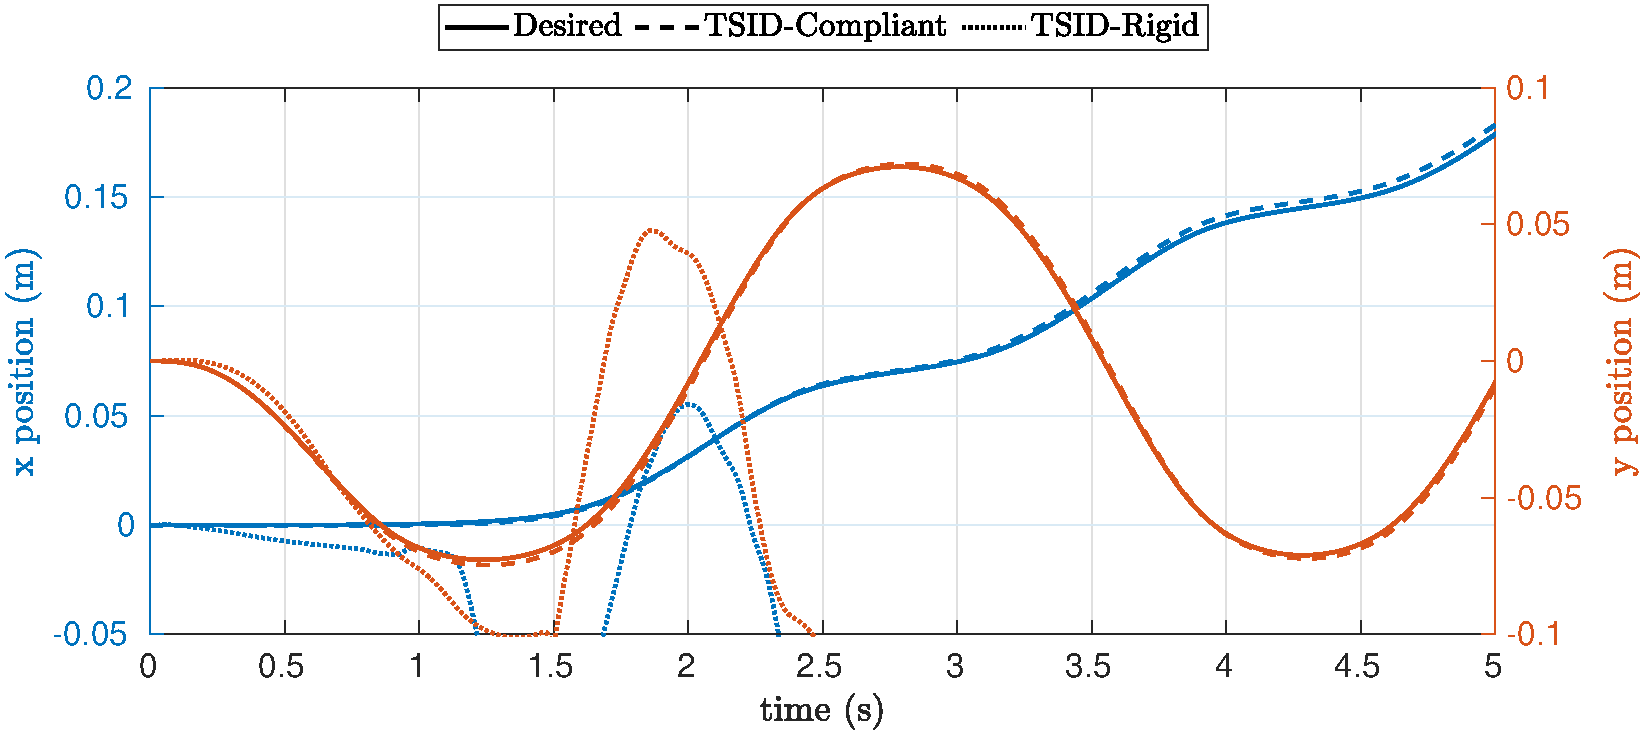
\includegraphics[height=0.151\textheight]{chapter_compliant_contact/figures/compliant_1e6_1e4_3_stiff_1e6_1e4_2_com.pdf}
        \caption{CoM}
        \label{fig:1e6_1e4_com}
    \end{subfigure}
    \hfill
    \begin{subfigure}[b]{0.49\textwidth}
        \centering
        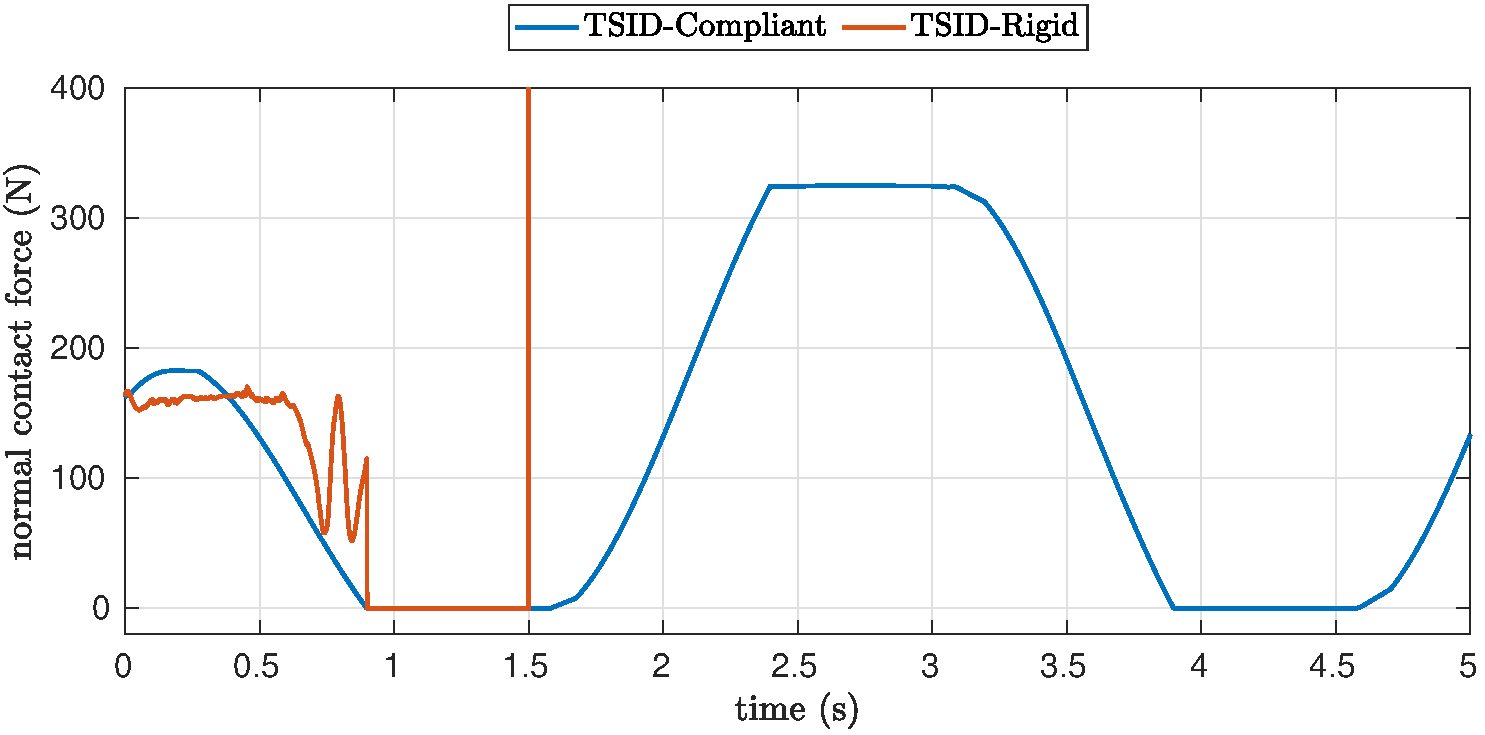
\includegraphics[height=0.151\textheight]{chapter_compliant_contact/figures/compliant_1e6_1e4_3_stiff_1e6_1e4_2_force.pdf}
        \caption{Normal contact force}
        \label{fig:1e6_1e4_force}
    \end{subfigure}
    \hfill
     \begin{subfigure}[b]{0.49\textwidth}
        \centering
        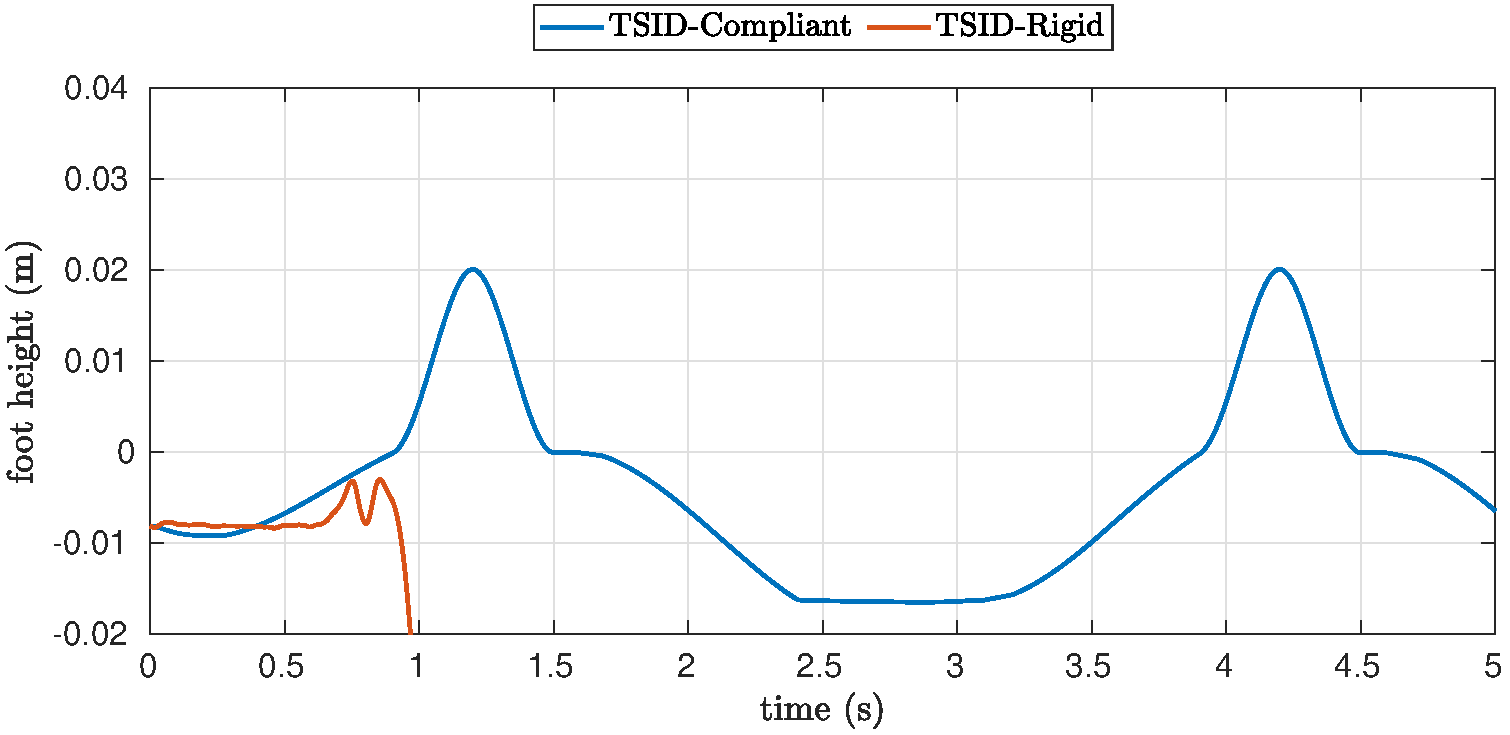
\includegraphics[height=0.151\textheight]{chapter_compliant_contact/figures/compliant_1e6_1e4_3_stiff_1e6_1e4_2_foot.pdf}
        \caption{Foot trajectory}
        \label{fig:1e6_1e4_foot}
    \end{subfigure}
    \end{myframe}
    \caption{Comparison between TSID-Rigid and TSID-Compliant. At $t\approx \SI{0.9}{\second}$, the TSID-Rigid makes the robot fall down.}
\end{figure*}
\begin{figure*}[t]
    \begin{myframe}{$k = \SI{8e6}{\newton \per \meter^3}$ $b = \SI{1e4}{\newton \second \per \meter^3}$}
        \centering
        \begin{subfigure}[b]{0.49\textwidth}
        \centering
        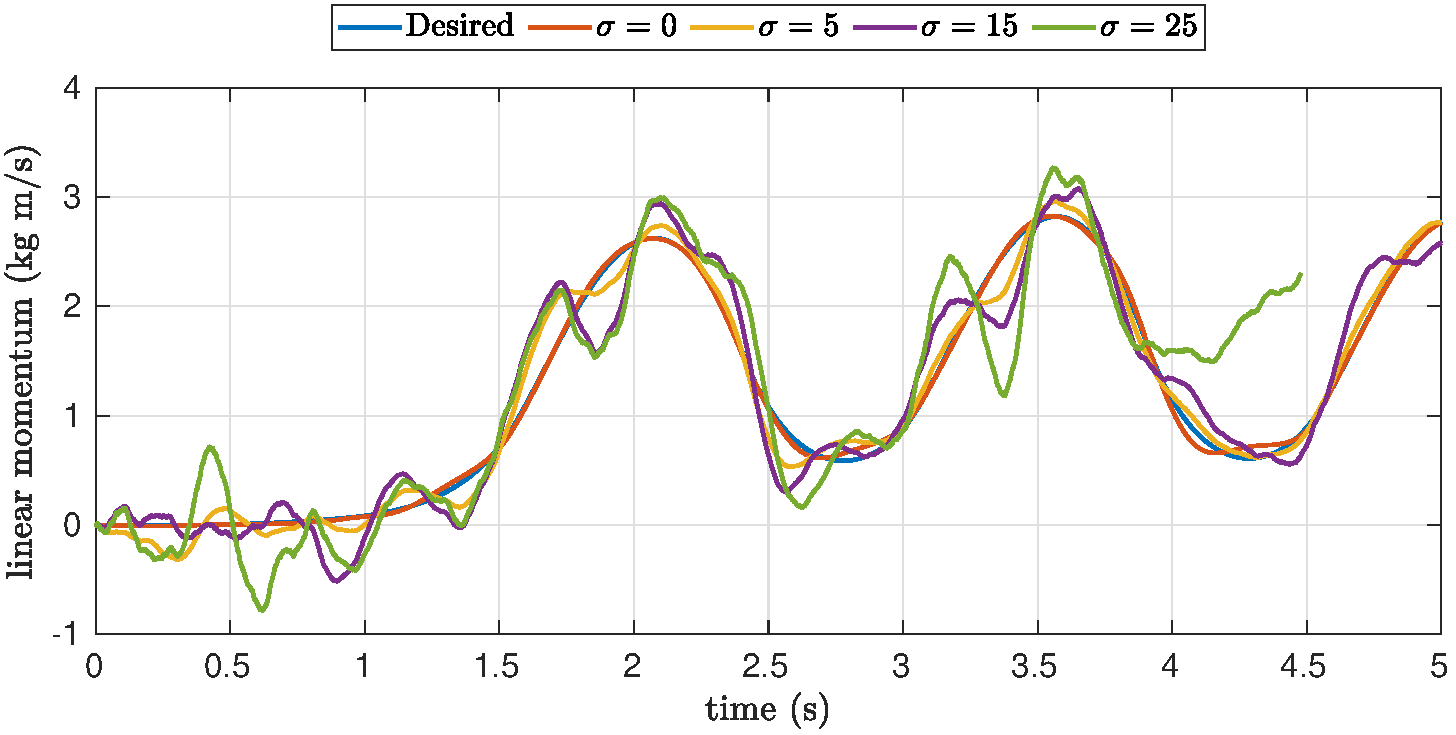
\includegraphics[height=0.151\textheight]{chapter_compliant_contact/figures/noise_linear_momentum_x.pdf}
        \caption{x coordinate}
        \label{fig:noise_linear_momentum_x}
    \end{subfigure}
    \hfill
    \begin{subfigure}[b]{0.49\textwidth}
        \centering
        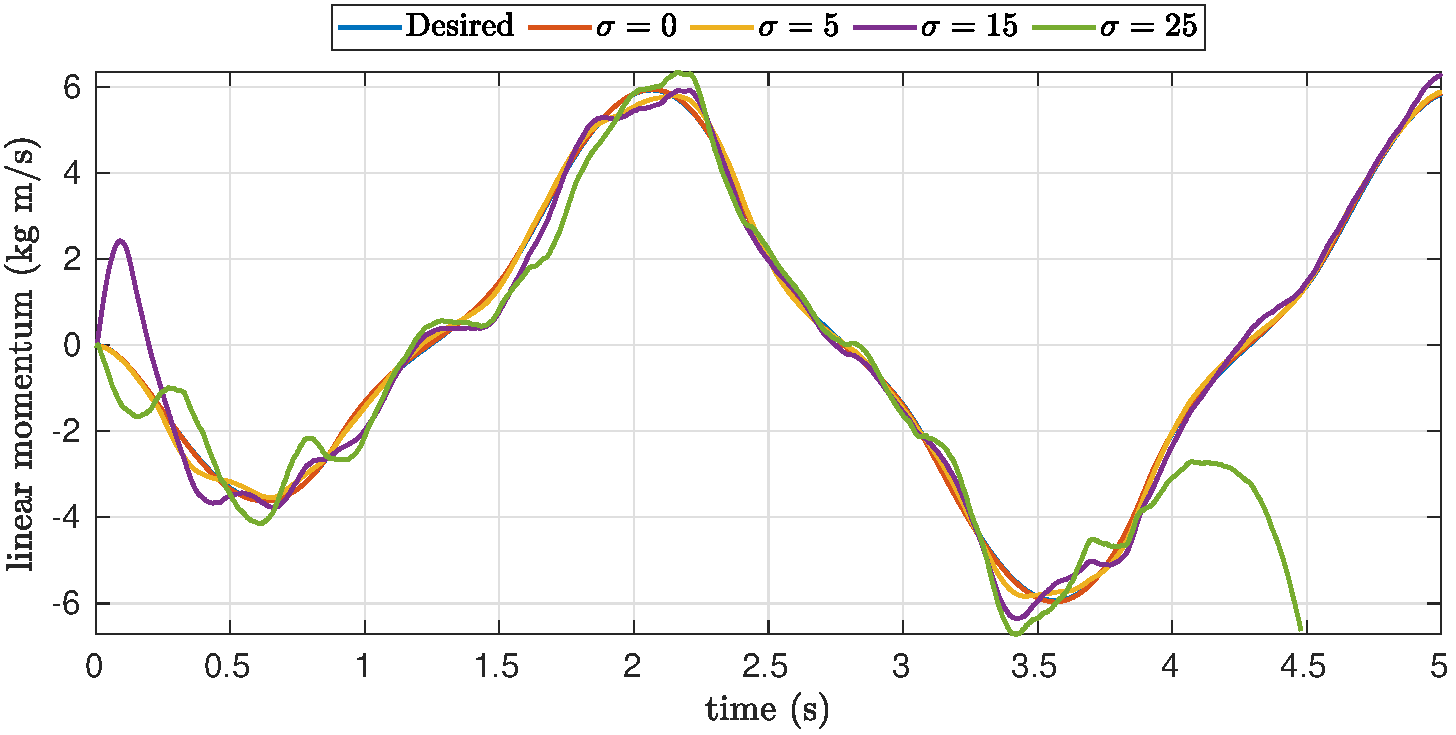
\includegraphics[height=0.151\textheight]{chapter_compliant_contact/figures/noise_linear_momentum_y.pdf}
        \caption{y coordinate}
        \label{fig:noise_linear_momentum_y}
    \end{subfigure}
    \hfill
     \begin{subfigure}[b]{0.49\textwidth}
        \centering
        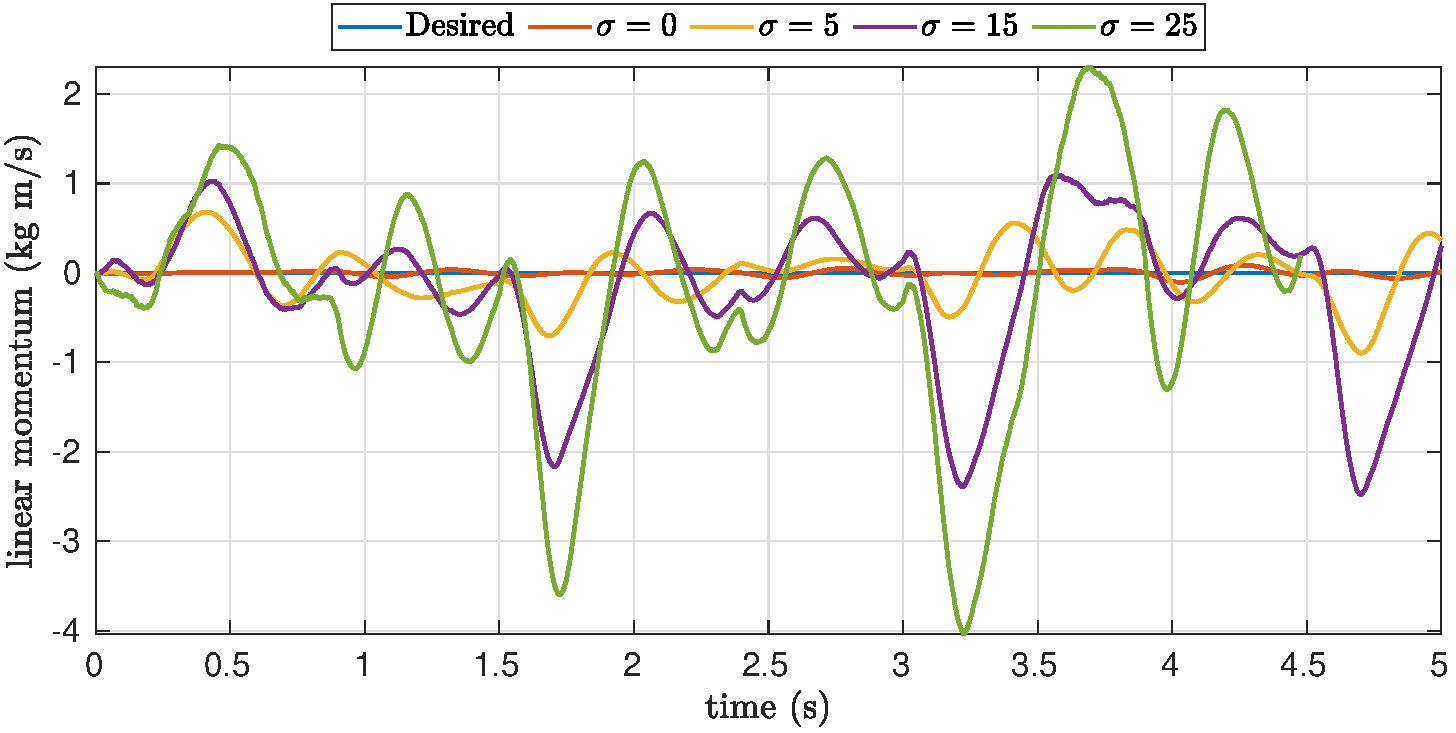
\includegraphics[height=0.151\textheight]{chapter_compliant_contact/figures/noise_linear_momentum_z.pdf}
        \caption{z coordinate}
        \label{fig:noise_linear_momentum_z}
    \end{subfigure}
    \end{myframe}
    \caption{Linear momentum tracking for different values of $\sigma$. At $t\approx\SI{4}{\second}$ and $\sigma = 20$  the robot fall down. \label{fig:noise_linear_momentum}}
\end{figure*}

\begin{figure*}[!t]
    \begin{myframe}{Contact parameter estimation}
    \centering
        \begin{subfigure}[b]{0.49\textwidth}
        \centering
        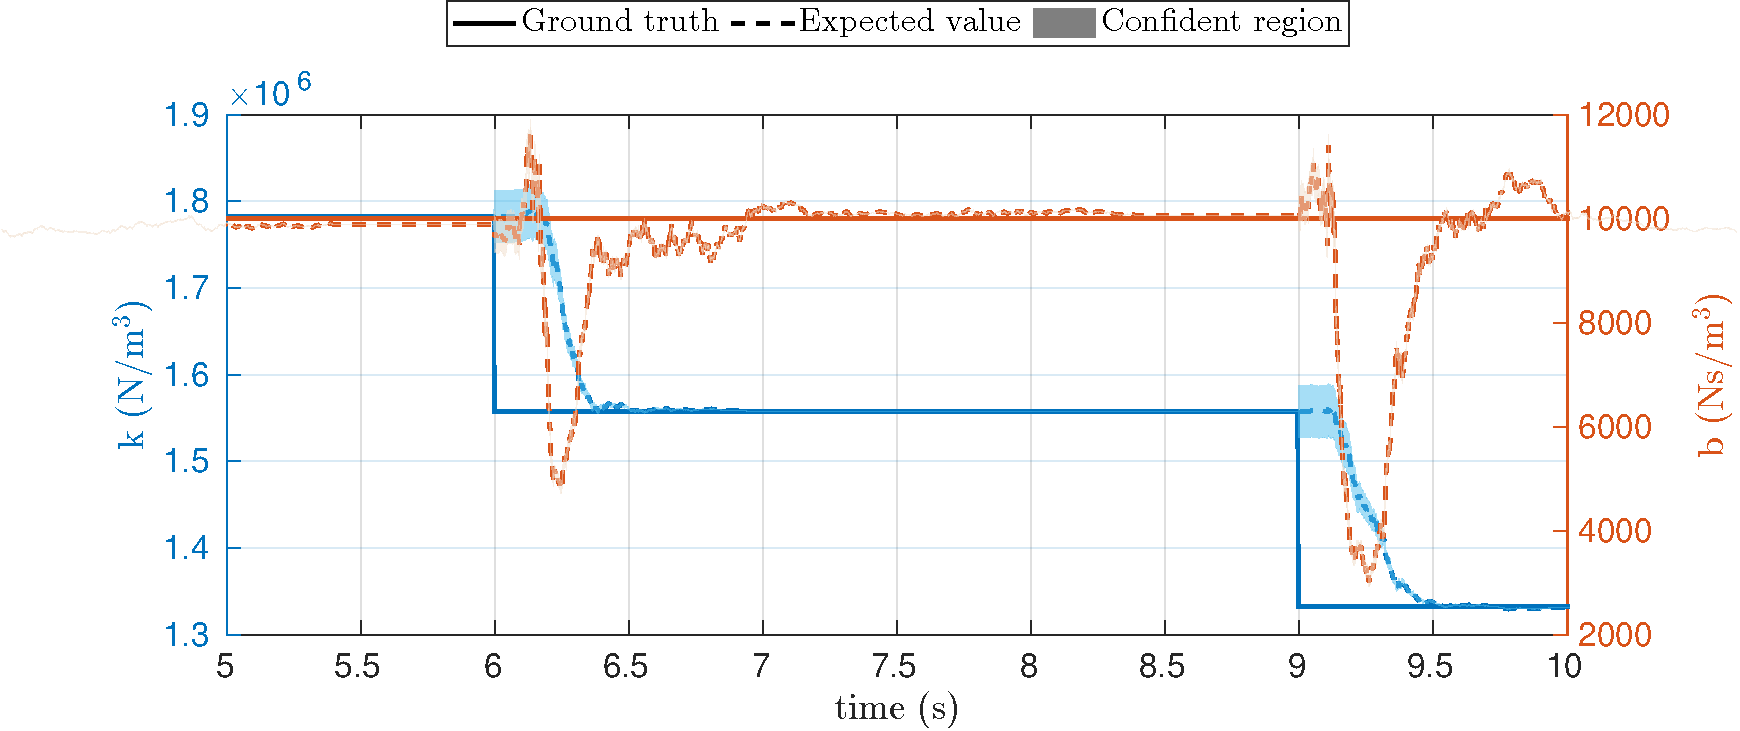
\includegraphics[height=0.141\textheight]{chapter_compliant_contact/figures/compliant_spring_varing_rls.pdf}
        \caption{Fixed $b$ and varying $k$}
        \label{fig:compliant_spring_varing_rls}
    \end{subfigure}
    \hfill
    \begin{subfigure}[b]{0.49\textwidth}
        \centering
        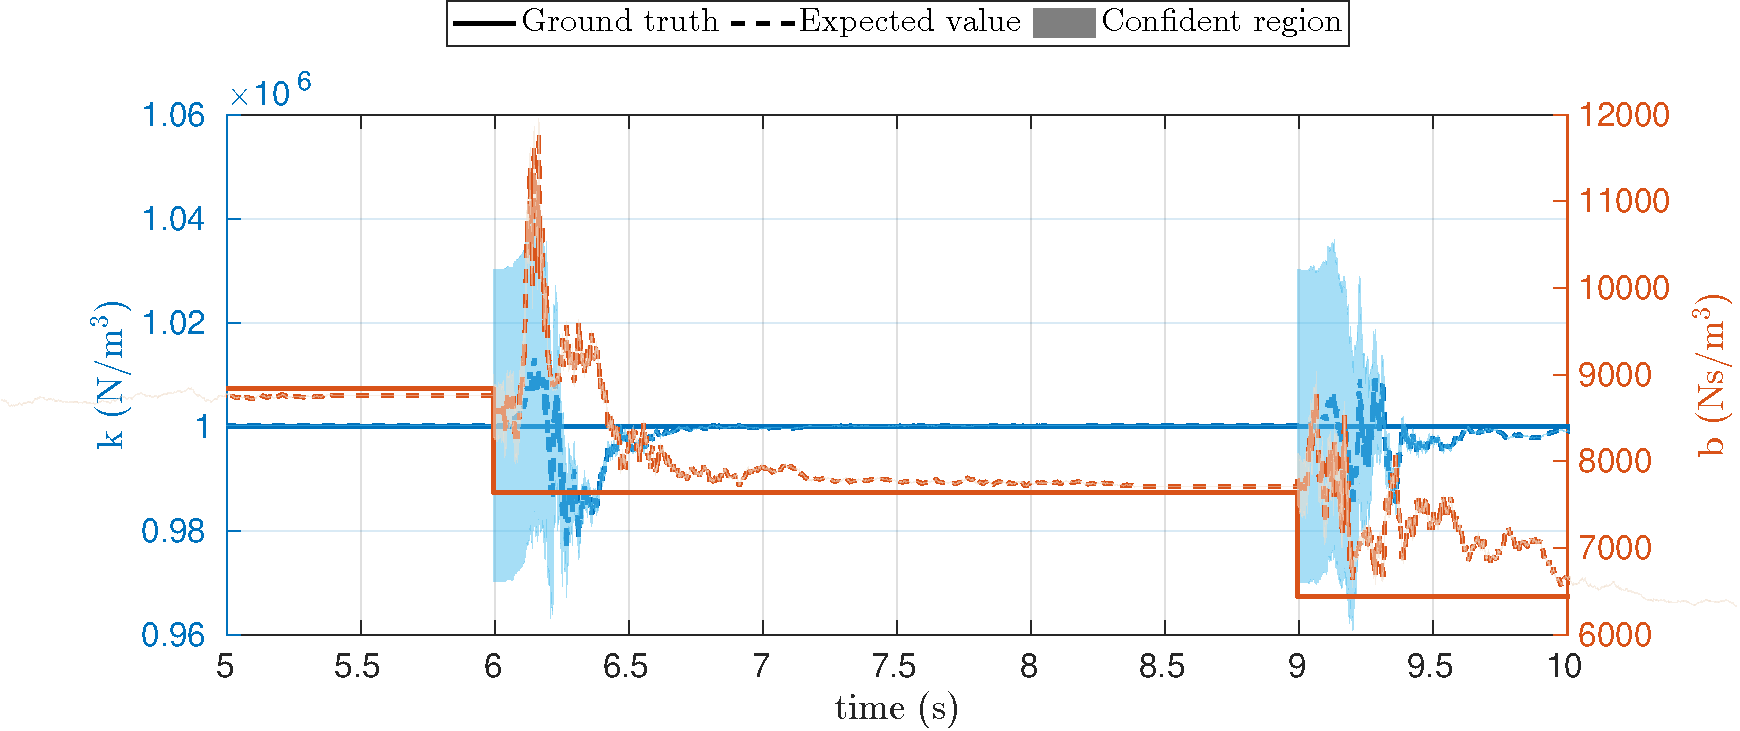
\includegraphics[height=0.141\textheight]{chapter_compliant_contact/figures/compliant_damper_varing_rls.pdf}
        \caption{Fixed $k$ and varying $b$}
        \label{fig:compliant_damper_varing_rls}
    \end{subfigure}
     \begin{subfigure}[b]{0.49\textwidth}
        \centering
        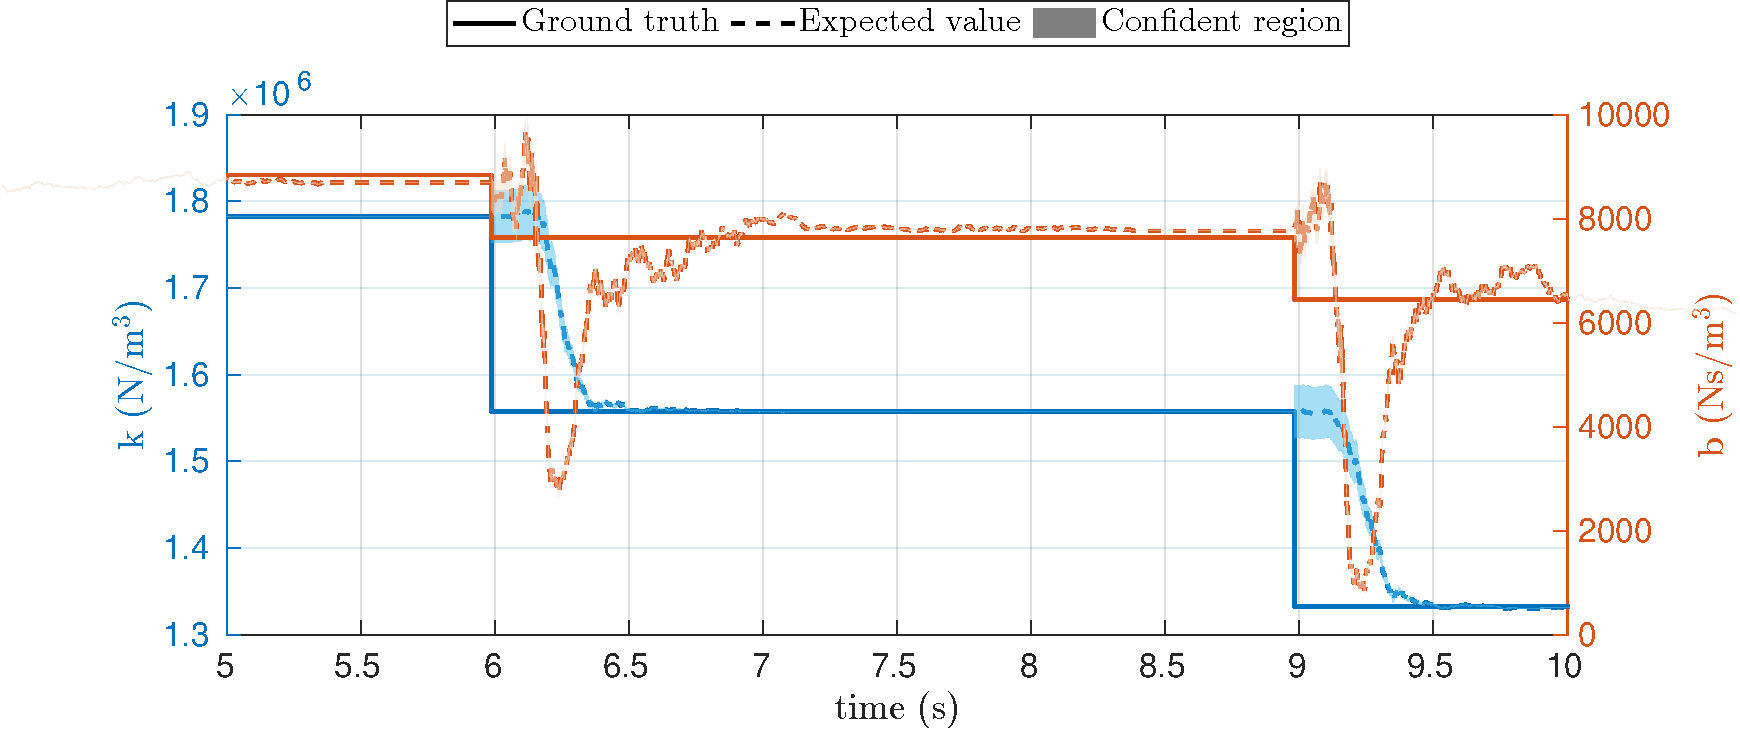
\includegraphics[height=0.141\textheight]{chapter_compliant_contact/figures/compliant_spring_damper_varing_rls.pdf}
        \caption{Varying $k$ and $b$}
        \label{fig:compliant_spring_damper_varing_rls}
    \end{subfigure}
    \end{myframe}
    \caption{Estimation of the contact parameters. The contact wrench is perturbed with zero-mean Gaussian noise with $\sigma = 5$.}
\end{figure*}




\subsubsection{Experiment 1} 
Figure~\ref{fig:2e6_1e4_com}  depicts the CoM tracking performance obtained with the TSID-Compliant and the TSID-Rigid. Both controllers seem to show good tracking performances, and the CoM error is kept below $\SI{1}{\centi \meter}$ in both cases. Note that the TSID-Rigid controller induces faster variations in the measured contact wrenches -- Figure~\ref{fig:2e6_1e4_force}. This contributes to the overall higher vibrations of the robot. One reason for this behavior is that the TSID-Rigid assumes full control on the desired contact wrenches. This assumption is generally valid for stiff contacts, but it does not hold if the environment is compliant. Figure~\ref{fig:2e6_1e4_foot} presents the left foot trajectory when the whole-body controller is either TSID-Compliant or TSID-Rigid. The TSID-Compliant ensures a smoother foot motion when it is in contact with the environment ($\SI{1.5}{\second}<t<\SI{3.5}{\second}$). 


\subsubsection{Experiment 2} 
There is no significant difference between the CoM tracking obtained with the two implementations of the whole-body controller -- Figure~\ref{fig:2e6_1e3_com} for $t < \SI{1}{\second}$. However, the lower the damper parameter $b$, the higher the acceleration required to change the contact wrench. This contrasts with the assumption of zero-foot accelerations of the TSID-Rigid controller -- see Equation~\eqref{eq:holonomic_constraint}. Consequently, the TSID-Rigid generates fast vibrations of the measured contact wrench and on the foot position -- Figures~\ref{fig:2e6_1e3_force} and \ref{fig:2e6_1e3_foot}, respectively. Clearly, these poor performances induce a bad tracking of the CoM shown in Figure~\ref{fig:2e6_1e3_com} at $t\approx \SI{1.5}{\second}$, and consequently the robot falls down. A possible solution to mitigate this problem is to increase the CoM gain in the TSID-Rigid controller. This unfortunately gives rise to higher robot oscillations, which in turn degrade the CoM tracking, and still the robot falls, or even worse, the controller may not be able to find a feasible solution.
\subsubsection{Experiment 3} 
The CoM tracking problem presented in Experiment 2 worsens at lower values of the contact parameter $k$.
Figure~\ref{fig:1e6_1e4_com} shows the CoM tracking performances of the two controllers. The TSID-Compliant is still capable of ensuring good performance. On the other hand, the TSID-Rigid generates faster variations on the measured contact wrenches and foot positions -- Figures~\ref{fig:2e6_1e4_force} and ~\ref{fig:2e6_1e4_foot}, respectively. Consequently, the controller, to maintain balance, requires high variations of the joint accelerations and at $t\approx\SI{0.9}{\second}$ fails while searching for feasible joint torques. Although tuning the TSID-Rigid controller may mitigate this problem, we were only able to postpone the failure. 

\subsection{Robustness of the TSID-Compliant}
In this section, we present the robustness capabilities of the TSID-Compliant controller in case of non-parametric uncertainty in the contact model.

We model the non-parametric uncertainty by using an \emph{additive white Gaussian noise}. So, the contact wrench acting on the robot becomes $f_k^m = f_k + \epsilon$, where $\epsilon$ is sampled from a Gaussian distribution with zero mean and standard deviation $\sigma$. $f$ is the contact wrench computed with the contact model~\eqref{eq:contact_model}.
Figure~\ref{fig:noise_linear_momentum} shows the linear momentum tracking performance obtained with different values of $\sigma$. The experiments are performed in the case of $k = \SI{8e6}{\newton \per \meter^3}$ and $b = \SI{1e4}{\newton \second \per \meter^3}$, however, similar considerations hold for the other sets of parameters -- see Table~\ref{tab:architecture_outcome}. 
The higher $\sigma$, the higher is the tracking error. The controller is capable of guaranteeing good tracking performance for all $\sigma < 20$. Indeed, at $\sigma = 20$ the controller is no longer able to guarantee acceptable performances and at $t\approx\SI{4}{\second}$ the robot falls down. 


\subsection{Anisotropic environment}
In this section, we show the performance of the contact parameter estimator in the case of an anisotropic environment. 
We model the contact parameters as a piecewise function of the forward walking direction assuming that all points of the contact surface have the same contact parameters. Also, to further test the robustness of the estimator, we add a zero-mean Gaussian noise (with standard deviation $\sigma = 5$) to the contact wrench.
To deal with contact parameter discontinuities, we reset the state covariance in the recursive least squares algorithm \citep{Colman2006OnDiscontinuities}. Each time a foot impacts the ground, the covariance is reset to the initial value. 
Figure~\ref{fig:compliant_spring_varing_rls} shows the performance of the estimator in the case of $b=\SI{1E4}{\newton\second\per\meter^3}$ and a space-dependent $k$. The discontinuity on the ground truth ($t\approx\SI{6}{\second}$ and $t\approx\SI{9}{\second}$) occurs when the swing foot makes contact with the environment. The observed parameters converge to the ground truth in less than a second.
The accompanying video shows that during the transient phases (e.g. $t\approx\SI{6.5}{\second}$), the controller achieves good overall performance.
Similar considerations hold in the case $k=\SI{1e6}{\newton\per\meter^3}$ and varying $b$ -- Figure~\ref{fig:compliant_damper_varing_rls} and space varying $k$ and $b$ -- Figure~\ref{fig:compliant_spring_damper_varing_rls}.